\section{Toelating van samengestelde knopen en satellieten}

Uit de voorgaande secties is duidelijk geworden onder welke omstandigheden men moet overgaan tot niet-torusknopen (samengestelde knopen~\cite{Faddeev1997KnottedSolitions}): zodra
één enkele torusknoop het vereiste aantal nucleonen niet meer stabiel kan binden. Dit kan optreden bij:

% --- Figuur 8: Satellietknoopconfiguratie ---
\begin{figure}[H]
    \centering
    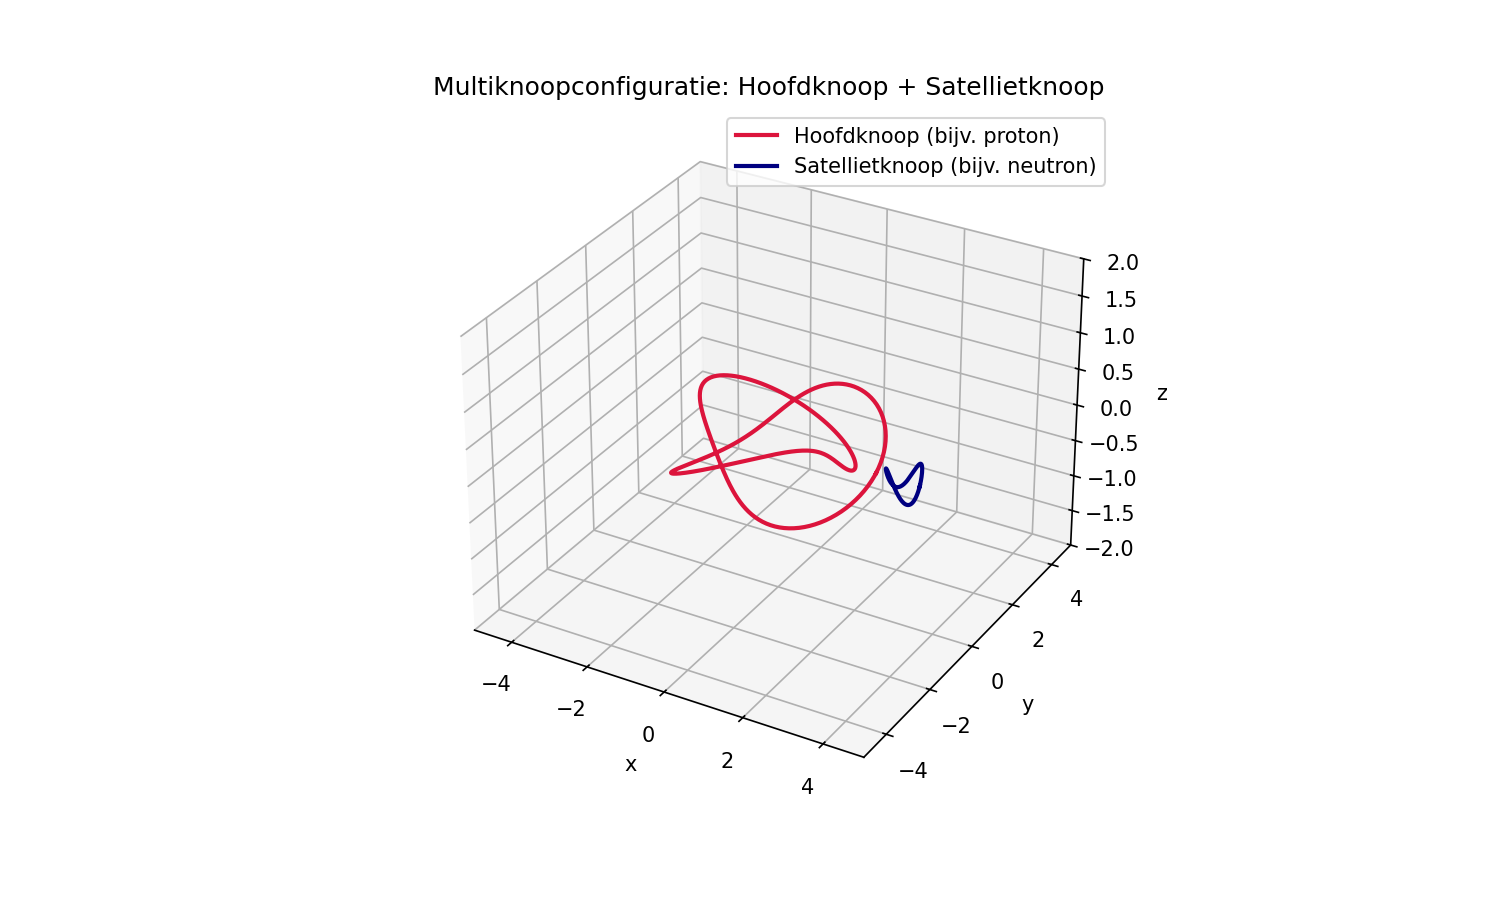
\includegraphics[width=0.7\textwidth]{../8_multiknoop}
    \caption{Voorstelling van een samengestelde vortexstructuur met één hoofd- en één satellietknoop (bijv. proton + neutronbinding zoals in deuterium).}
    \label{fig:satellietknoop}
\end{figure}

\begin{itemize}
    \item \textbf{Te hoge lading:} Wanneer $Z$ groot wordt, groeit de benodigde heliciteit en dus rotatie-energie ~ met $Z$. Uiteindelijk wekt de knoop zóveel centrifugale spanning op dat de ætherdruk niet langer alle protonen bijeen kan houden. Dit is het punt waarop extra protonen eerder een afzonderlijke knoop gaan vormen dan de bestaande knoop verder uit te rekken. In het periodiek systeem is dit zichtbaar rond de overgang van middellange naar zware elementen, waar extra protonen minder stevig gebonden raken (snelle toename van instabiliteit en radioactiviteit bij toenemend $Z>82$). VAM geeft hier een topologische verklaring: boven een kritisch $L_k$ is er een energetische bifurcatie waarbij $L_k$ zich opsplitst in $L_{k1}+L_{k2}$ met lagere individuele waarden. Daarom wordt bijvoorbeeld lood ($Z=82$) nog net door één knoop gehouden, maar bismut ($Z=83$) is al licht radioactief – een hint dat de knoop begint over te gaan naar een 2-knopensysteem.

    \item \textbf{Teveel neutronen:} Neutronen ($N$) verhogen de massa (dus dragen bij aan onderdrukkende druk), maar als $N$ aanzienlijk groter wordt dan $Z$, neemt de stabiliserende werking af. Op een gegeven moment kunnen extra neutronen niet meer netjes als kleine twistjes of satellietjes in de knoopstructuur worden opgenomen en gaan ze zich groeperen tot eigen subknoopjes. Empirisch zien we dat zeer neutronrijke nuclei clustervorming vertonen of gemakkelijk in fragmenten uiteenvallen. In VAM-termen: als neutronsatellieten onvoldoende koppeling met de hoofdknoop hebben, kunnen ze samen een losse vortexring vormen en afsplitsen.

    \item \textbf{Energetisch criterium:} Formeel zou men een energievergelijking kunnen opstellen: één knoop is stabiel zolang $E_\text{knoop}(Z,N) < E_\text{deling}(Z,N)$, waarbij rechts een configuratie is met twee of meer knopen die samen $Z,N$ verdelen. Wanneer $E_\text{deling} < E_\text{knoop}$, zal samenstelling prefereren. VAM biedt een manier om $E$ te schatten via integralen over $\omega^2$ (vortexenergie) en druktermen. Hoewel een volledige berekening beyond scope is, kan men kwalitatief stellen dat $E_\text{knoop}$ groeit ongeveer als $L_k^2$ (want meer heliciteit geeft disproportioneel meer energie), terwijl door splitsing $L_k$ verdeeld wordt en de energie ~ als som van kwadraten van kleinere getallen komt. Bijvoorbeeld $L_k=10$ vs twee knopen $L_{k1}=5, L_{k2}=5$: $10^2 =100$ vs $5^2+5^2=50$ in arbitraire eenheden – dus splitsing zou de helft van de energie kunnen schelen. Dit zeer simplistisch model laat zien dat boven een zekere heliciteit splitsing enorm voordelig wordt. Daarom is het bestaan van superzware stabiele knopen uitgesloten; de natuur kiest daar composieten.
\end{itemize}

Gezien deze inzichten concluderen we dat niet-torusknopen nodig worden bij zware nuclei. Hieronder verstaan we zowel samengestelde knopen (waar twee of meer prime-knopen verbonden zijn in één configuratie, vergelijkbaar met hoe een gecomponeerde knoop in de topologie gedefinieerd is als de connect-sum van twee knopen) als satellietknopen (waar een kleine knoop \grqq gebonden\textquotedblright is rondom een grotere, vergelijkbaar met een knoop om een streng binden).

Een samengestelde knoop binnen VAM zou kunnen corresponderen met b.v. een kern bestaande uit twee gelinkte vortexlussen – elke lus mogelijk zelf geknoopt. Dit zou toepasbaar kunnen zijn op relatief symmetrische splitsingen, zoals $^{20}$Ne dat gezien kan worden als 5 alfa's (5 kleine knopen) samen, of $^{236}$U dat prompt in twee composietknopen (rond massagetal 120 elk) uiteen kan vallen.

Een satellietknoop is conceptueel geschikt om een enkel of enkele neutronen te modelleren die een kern omringen (bijvoorbeeld $^3$He versus $^4$He, waar $^4$He een extra kleine vortexring gekoppeld heeft). Deze satelliet deelt dan wel de stroming (en is dus gebonden via Bernoulli-onderdruk), maar is topologisch een apart lusje om de hoofdtorus. Bij teveel satellieten ontstaat een gecompliceerd vlechtwerk (netwerk van fluxen) dat eventueel gereconfigureerd kan worden.

Men kan dus zeggen: Zodra de eenvoudigste torusknoop niet alle nucleonen binnen één topologie kan omvatten, schakelt de natuur over op een hiërarchie van knopen – van hogere $p$ tot uiteindelijk multiknoop. Dit is een fascinerende multiscalar emergentie: de atoomkern is geen monolithisch bolletje, maar een knoop van knopen van fluïdum!